\documentclass[output=paper]{LSP/langsci} 
\author{Ana Ruth Moresco Miranda\affiliation{Universidade Federal de Pelotas}\lastand 
João Veloso\affiliation{Faculdade de Letras da Universidade do Porto\\Centro de Linguística da Universidade do Porto (FCT-UID/LIN/0022/2016)}
}
\title{Consciência linguística: aspetos fonológicos}
\abstract{}
\ChapterDOI{10.5281/zenodo.889467}
\maketitle
\begin{document}
\section{Aquisição da linguagem, desenvolvimento fonológico e desenvolvimento das capacidades metafonológicas}\is{conhecimento!metafonológico}
\label{sec:miranda_aquisicao}

A aquisição da linguagem, especificamente o desenvolvimento fonológico, é um processo paradoxalmente simples e complexo. A complexidade deriva do tipo de conhecimento envolvido, o qual engloba um conjunto intrincado de informações melódicas e prosódicas que devem estar articuladas para que a produção linguística das crianças se realize. Já a simplicidade está relacionada com a forma natural e espontânea com que a criança, desde as primeiras palavras, lida com esses elementos que integram a segunda articulação da linguagem.

Bem antes de os estudos psicolinguísticos começarem a ser desenvolvidos, na segunda metade do século XX, pesquisadores da linguagem já demonstravam interesse pela aquisição linguística e expressavam ideias importantes a respeito do tema. \citet{humboldt}, no seu tratado sobre a linguagem, concluiu que não se pode ensinar uma língua, mas apenas apresentar as condições para que ela se desenvolva de modo espontâneo, com a sua especificidade própria, na mente dos sujeitos. Tal afirmação está na base da proposta chomskiana que impulsionou os estudos psicolinguísticos referentes ao desenvolvimento da linguagem. Bühler, por seu turno, na epígrafe do clássico de Jakobson \citetitle{jakobson1941} \citeyearpar{jakobson1941}, pôs em evidência a relevância dos dados de aquisição ao escrever que a criança oferece a única oportunidade que temos para observar a linguagem no seu estado nascente.

Os estudos em \isi{aquisição fonológica} têm mostrado unanimemente que o conhecimento implícito sobre a estrutura e o funcionamento do nível fonológico\is{conhecimento!fonológico} vai sendo forjado ao longo dos primeiros anos de vida da criança. A construção desse conhecimento pode ser observada tanto nas respostas dadas pelos aprendentes -- em períodos nos quais a sua produção linguística ainda é bastante distinta da do adulto, com demonstrações de que a capacidade de perceção precede a de produção --, como nas formas iniciais produzidas por eles (versões próprias surgidas a partir da interação de um mecanismo geral para a construção de gramáticas e partindo do \textit{input} disponível na comunidade linguística de que fazem parte).

Esta assimetria entre produção e perceção fonológica, designada na literatura como Fenómeno fis, teve o nome cunhado a partir de um diálogo entre uma criança e um adulto, conforme relatado no artigo \textit{Psycholinguistic research methods} \citep{berkobrown1960} e reproduzido em (\ref{ex:miranda_berkobrown}).

\ea\label{ex:miranda_berkobrown}
Criança: ``\textipa{[\textprimstress fiS]}'' (em referência a seu peixe de plástico inflável, \textit{fish}).\\
Adulto: ``É este o teu \textipa{[\textprimstress fis]}?''\\
A criança rejeita a declaração.\\
Adulto: ``É este o teu \textipa{[\textprimstress fiS]}?''\\
Criança: ``Sim, o meu \textipa{[\textprimstress fiS]}.''
\z

Nota-se, pelo diálogo, que a criança, embora não produza a fricativa [$-$anterior], já percebe o contraste existente no seu sistema materno. Esse comportamento é interpretado como uma evidência de que, embora ela não possa ainda produzir o fonema \textipa{/S/}, pode percebê-lo como distinto de \textipa{/s/}. Há reiterados exemplos semelhantes a esse descritos em várias línguas já estudadas. Um exemplo análogo do português, referente à palavra ‘gan\textipa{[S]}o’ produzida pela criança como ‘gan\textipa{[s]}o’, foi registado por \citet{matzenauer1988}.\footnote{Comunicação pessoal (dados recolhidos pela autora para a sua dissertação de mestrado – \citealt{matzenauer1988}).}
\citet{berti2006}, num estudo realizado sobre as fricativas, adiciona elementos à discussão sobre a relação produção/perceção, trazendo evidências acústicas de que as trocas entre segmentos, no caso das fricativas [$\pm$anterior], são, na verdade, \textit{contrastes encobertos}, já que os parâmetros acústicos característicos de um e de outro segmento podem ser detetados, embora com base na observação auditiva não se possa escutar o contraste nas produções infantis.

O património fonológico da criança pode ser observado ainda em revelações das suas habilidades epilinguísticas, as quais derivam do conhecimento implícito já construído e denotam algum controle cognitivo sobre ele. Os exemplos apresentados em (\ref{ex:miranda_2}),\footnote{Dados coletados por Ana Ruth Moresco Miranda.} recolhidos em crianças em fase de aquisição do português do Brasil, foram produzidos por crianças com idades de 2:10 e 2:05, respetivamente.

\ea\label{ex:miranda_2}
 \ea{
Valentin: A tia comprou vinho porquê?\\
Prima: Para beber.\\
Valentin: Eu não tomo vinho\ldots eu como ovinho\ldots é bem fresquinho.
}
\ex{
Mãe: Olha a lua, que linda.\\
Gonçalo: Mãe, lua parece com rua.
}
\z
\z

As duas produções das crianças são exemplos de que, em idades bem precoces, a sensibilidade\is{sensibilidade fonológica} fonémica pode ser observada. Nos dois comentários espontâneos, podemos observar algum tipo de reflexão linguística. O primeiro exemplo mostra uma atividade de subtração de fonema\is{subtração fonémica} (`vinho' por `ovinho'); e o segundo, a \isi{substituição de fonema} (\textipa{/l/} por \textipa{/x/}). Tais dados revelam indícios de um tipo de consciência sonora\is{consciência!fonémica/segmental} cuja motivação é, possivelmente, advinda de práticas de \isi{letramento} das quais as crianças participam, provavelmente pelo contacto com músicas e poemas infantis, material rico em jogos de linguagem que exploram rimas e aliterações.

Tal sensibilidade\is{sensibilidade fonológica} manifesta-se graças ao conhecimento linguístico interiorizado a respeito do funcionamento da gramática sonora e pode envolver não apenas fonemas, mas também sílabas, conforme o exemplo do português europeu apresentado em (\ref{ex:miranda_3}).\footnote{Dados recolhidos por Maria João Freitas.}

\ea\label{ex:miranda_3}
Situação em que Laura (2 anos) descreve um desenho:\\
\textit{Mãe}: É uma\ldots\\
\textit{Laura}: É uma\ldots\\
\textit{Mãe}: cha\ldots\\
\textit{Laura}: miné\\
\textit{Mãe}: Agora diz\ldots\\
\textit{Laura}: chaminé\\
\textit{Mãe}: Outra vez\ldots\\
\textit{Laura}: \textit{cha}//\textit{mi}//\textit{né}
\z

Para \citet{gombert1992,gombert2003}, a um nível epilinguístico o controle\is{controlo!epilinguístico} exercido de forma automática sobre o processamento linguístico é propiciado pelo conhecimento implícito, mas não está disponível ao acesso consciente. O controle consciente,\is{consciência!linguística} característico de procedimentos metalinguísticos, somente poderá ser observado a partir do momento em que demandas externas ocorram. A aprendizagem da leitura e da escrita, de acordo com o autor, constitui um desses requisitos -- ou demandas \textit{externas} -- capazes de produzir pressão suficiente para que ocorra o monitoramento consciente no processamento da língua, compelindo a criança à reflexão sobre a linguagem oral.

O modelo de desenvolvimento de \citet{gombert1992,gombert2003} inclui dois tipos de controle: o epilinguístico\is{controlo!epilinguístico} e o metalinguístico.\is{controlo!metalinguístico} O autor propõe três fases para o desenvolvimento linguístico: a primeira é a fase de aquisição das habilidades linguísticas, que inclui o conhecimento implícito sobre a estrutura e o uso da linguagem; a segunda, de aquisição do controle epilinguístico\is{controlo!epilinguístico} em que o conhecimento linguístico é reorganizado em formato multifuncional, porém não acessível conscientemente; e a terceira, de aquisição do conhecimento metalinguístico desencadeada por demanda externa e controle intencional da organização estabelecida na fase 2.

Em relação ao conhecimento metalinguístico, pode considerar-se que a ele se associam três conceitos: \textit{intenção}, \textit{controle} e \textit{consciência}.\is{consciência!linguística} Para \citet[42]{cardosomartins1991}, a intenção e o controle em atividades linguísticas podem resultar numa reflexão sobre a língua ou, ainda, sobre estruturas que a compõem. No que diz respeito à fonologia, a Consciência Fonológica\is{consciência!fonológica} (CF) é um exemplo de habilidade metalinguística\is{controlo!metalinguístico} que pode ser definida como a capacidade de manipular as unidades de segunda articulação da língua, o que compreende as sílabas e seus constituintes e também os fonemas.

\citet{bradley1978} desenvolveram experimentos para testar a relação entre dificuldade de \isi{leitura} e consciência fonológica\is{consciência!fonológica} e concluíram que o desempenho em CF é um preditor robusto no que diz respeito à habilidade de \isi{leitura}. Desde então, diversos estudos experimentais foram realizados a fim de que a relação entre os níveis de CF e o desenvolvimento da \isi{leitura} e da \isi{escrita} pudesse ser verificada. De forma geral, a tendência nos estudos mais atuais é a de argumentar em favor de uma reciprocidade entre desenvolvimento de CF e habilidades de \isi{leitura}, pois o desenvolvimento da consciência sobre a estrutura sonora da língua,\is{consciência!fonológica} especialmente a consciência fonémica\is{consciência!fonémica/segmental} -- ou \textit{segmental} --, está vinculado à aprendizagem da \isi{leitura} e da \isi{escrita}, sobretudo em \isi{Sistemas de Escrita Alfabética}, e vice-versa.

\newpage Desde os estudos pioneiros conduzidos por José Morais e seus colaboradores (cf., entre outros: \citealt{alegriamorais1979,morais_etal1979,nakamura_etal1998}), abrangendo um vasto conjunto de línguas e sujeitos com diferentes graus de \isi{letramento},\footnote{Os principais grupos de sujeitos estudados por estas investigações repartem-se da seguinte forma: crianças em idade pré-escolar; crianças em fases iniciais da aprendizagem da \isi{escrita}; adultos iletrados; adultos letrados em SEA (``Sistema de Escrita Alfabética''); adultos letrados noutros sistemas de \isi{escrita}.} é ponto assente assumir-se que a consciência segmental\is{consciência!fonémica/segmental} é resultado do conhecimento da \isi{escrita} alfabética. Considera-se consciência segmental\is{consciência!fonémica/segmental} a operacionalização verificável dos segmentos consonânticos e vocálicos como unidades últimas da análise fónica sobre material verbal associada à capacidade de efetuar manipulações metafonológicas\is{conhecimento!metafonológico} explícitas que tomam o segmento fonológico como critério de aplicação.

Mais relevantemente, porém, não poderemos ignorar que o relacionamento entre a aquisição/desenvolvimento fonológico e a aprendizagem da \isi{leitura} e da \isi{escrita} deve ser encarado como um binómio \textbf{bidirecional}, conforme ilustra a Figura \ref{fig:miranda_1}.

\begin{figure}
  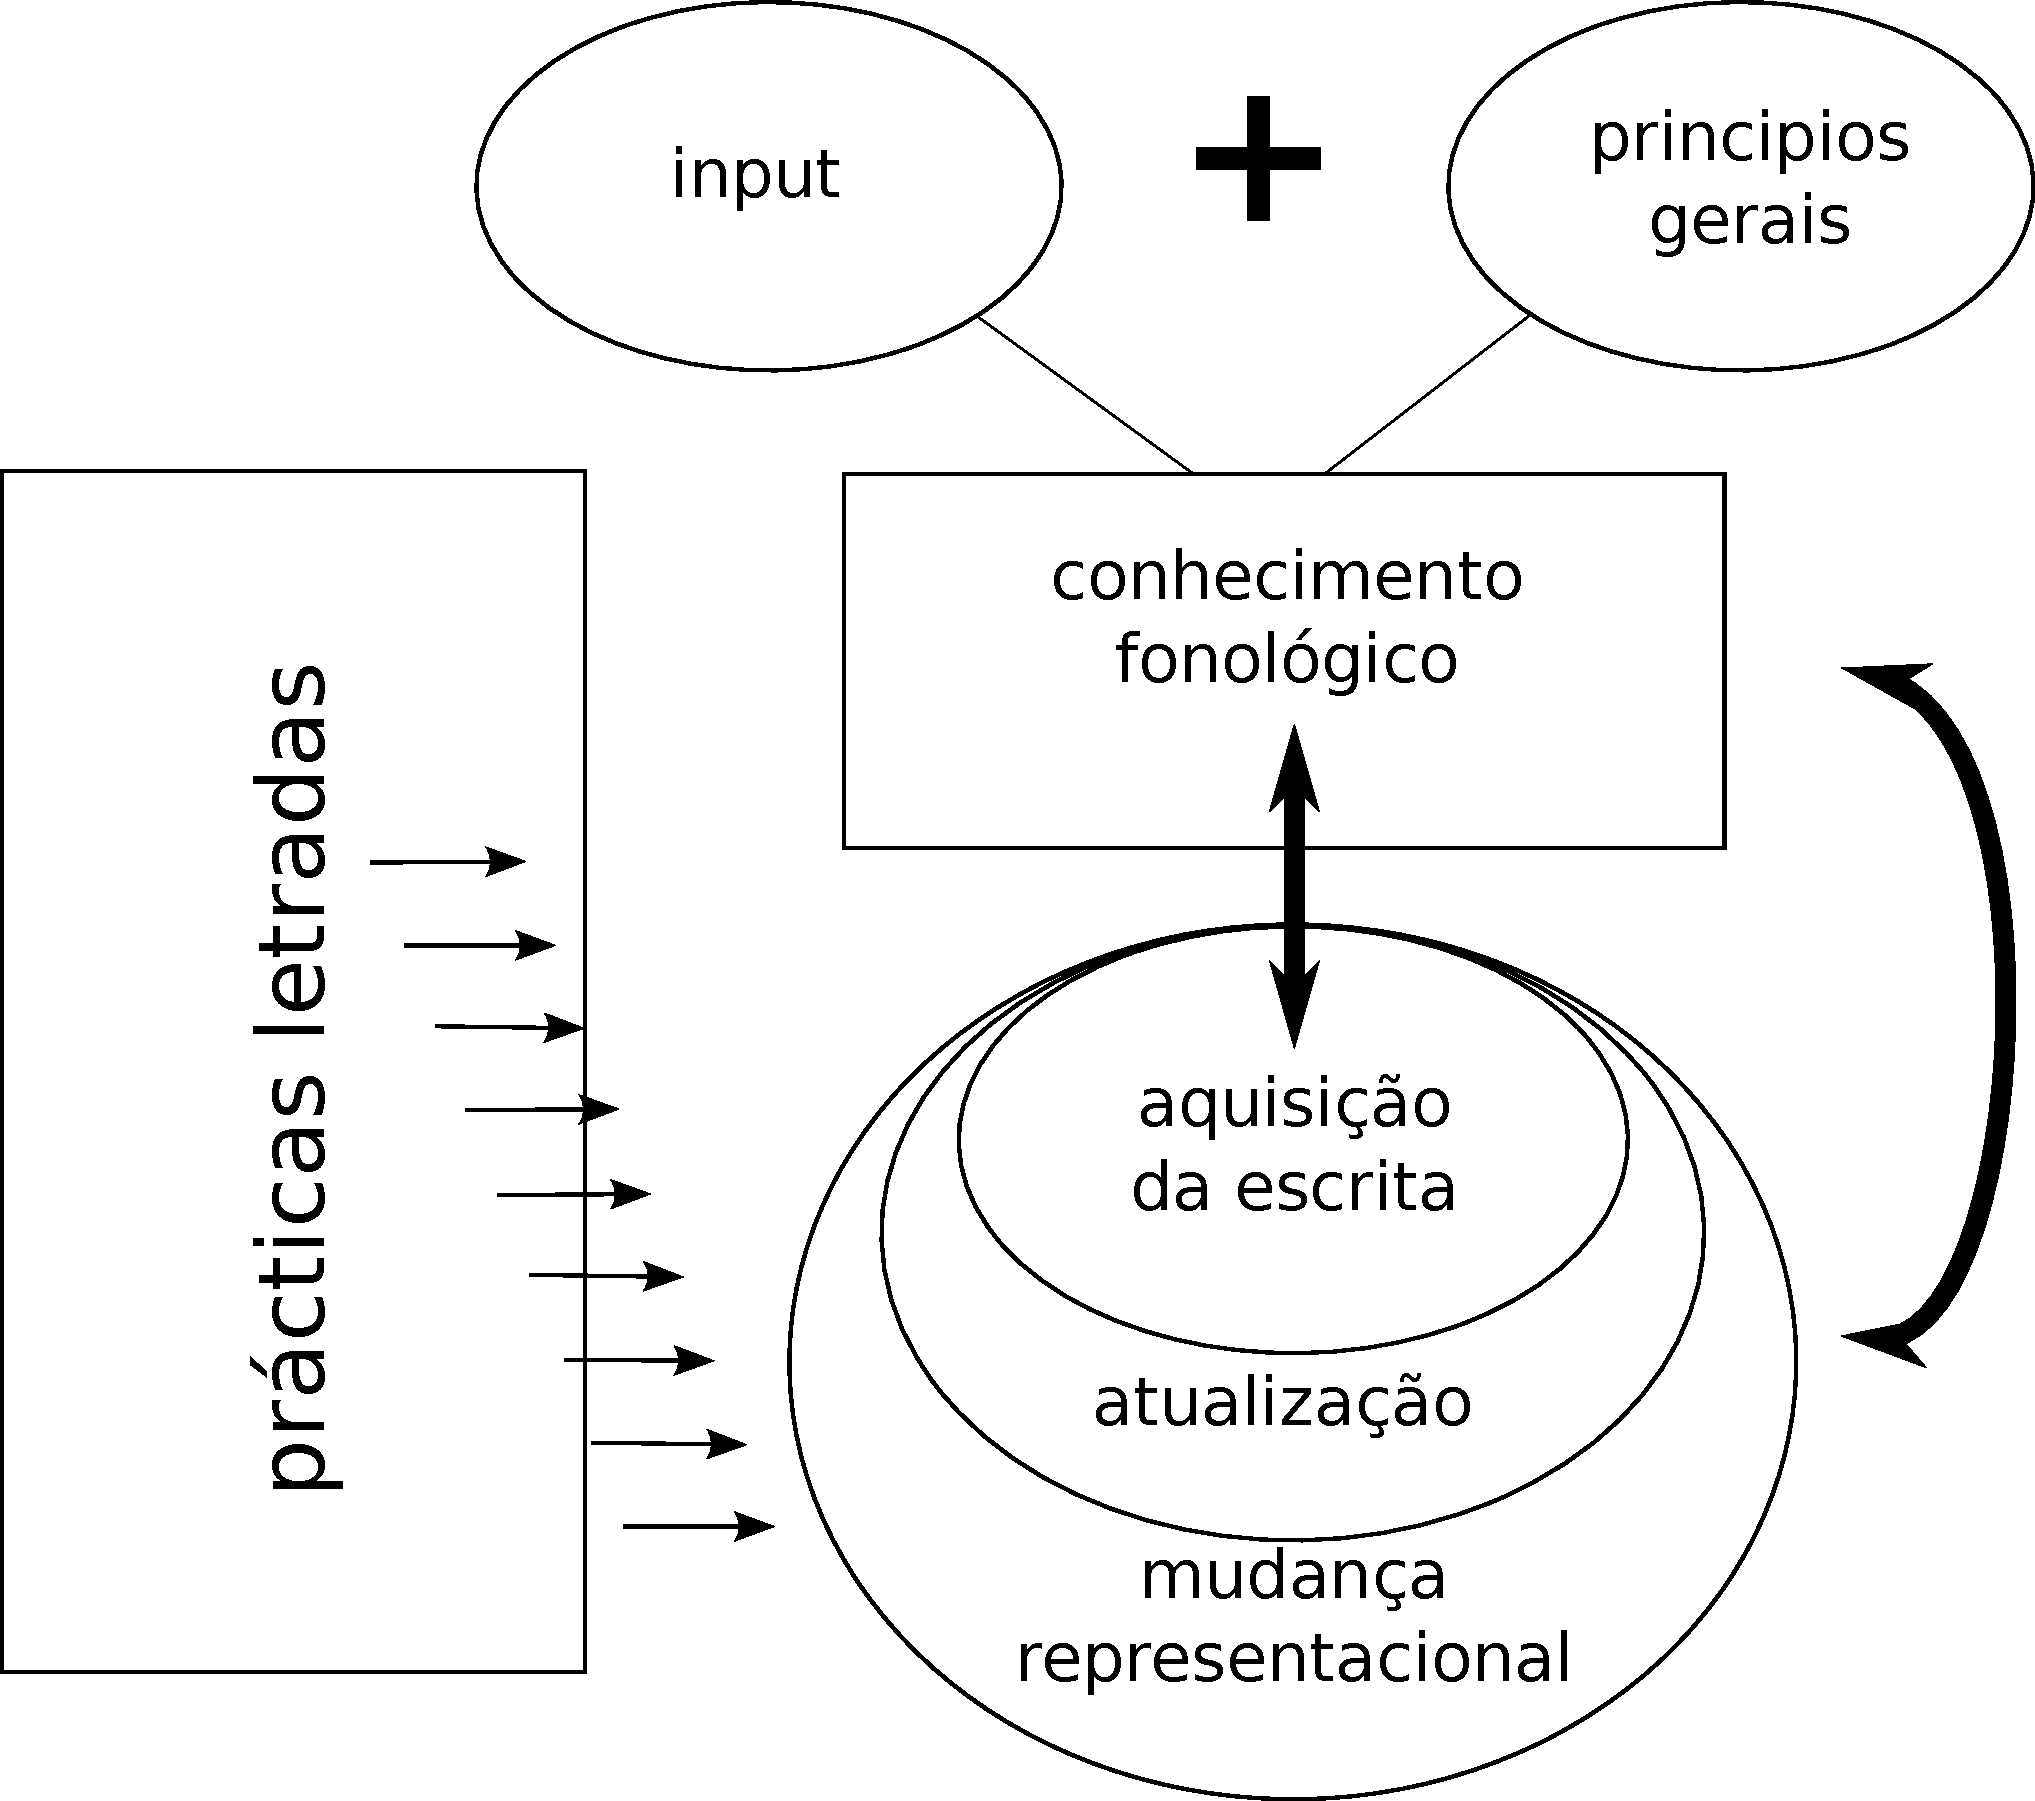
\includegraphics[height=.3\textheight]{figures/miranda_1.pdf}
  \caption{Bidirecionalidade do binómio aquisição/desenvolvimento fonológico e aprendizagem da \isi{leitura} e da \isi{escrita} \citep{miranda2014}}
  \label{fig:miranda_1}
\end{figure}

De acordo com esta perspetiva bidirecional, podemos dizer que:
\begin{itemize}
\item o conhecimento fonológico,\is{conhecimento!fonológico} de certa forma, alimenta a aprendizagem da \isi{leitura} e da \isi{escrita}. Bons resultados em tarefas como a \isi{identificação de rimas} \citep{seidenbergtanenhaus1979} e a segmentação silábica\is{segmentação!segmentação silábica} \citep{treimandanis1988,ventura_etal2001}, p. ex., são preditores de bom desempenho da aprendizagem da \isi{leitura} e da \isi{escrita};
\item simultaneamente, a aprendizagem da \isi{escrita} pode reformatar aspetos essenciais do conhecimento fonológico.\is{conhecimento!fonológico} É o que sucede, p. ex., no caso dos sujeitos expostos à aprendizagem de um Sistema de Escrita Alafabética (SEA), no que concerne ao desenvolvimento da sua consciência fonémica.\is{consciência!fonémica/segmental}
\end{itemize}

Considerando-se a dimensão fonológica da língua, é importante também levar em conta a diferença entre sensibilidade\is{sensibilidade fonológica} e consciência\is{consciência!fonológica} (cf. \citealt{bowey1994}). A primeira pode ser observada em exemplos como aqueles referidos em (\ref{ex:miranda_2}) e (\ref{ex:miranda_3}) ou em respostas a atividades que exigem apenas a deteção de similaridades e diferenças; a segunda é comprovada a partir de atividades que exigem manipulação deliberada e explícita de unidades fonológicas -- por exemplo, tarefas de isolamento de segmentos ou sílabas -- e que estão fortemente relacionadas com a compreensão dos princípios do SEA. Os dados apresentados em (\ref{ex:miranda_4}),\footnote{Exemplos de \citet[230,232]{rigatti2008}, obtidos durante a realização, no início do primeiro ano escolar, de um teste de consciência fonológica\is{consciência!fonológica} (CONFIAS, \citealt{moojen_etal2003}). Antes da pergunta descrita, a autora explicou a tarefa e deu exemplos às crianças.} colhidos em produções do português do Brasil e referentes às respostas a testes de CF aplicados a um aluno que ainda não está no nível alfabético de \isi{escrita}, ilustram a complexidade de uma tarefa que desafia a criança a separar forma sonora e significado.

\ea\label{ex:miranda_4}
\ea{
Pesquisadora: Se eu tirar o `pi' de `piolho', como fica?\\
Criança 1: `lêndea'
}
\ex{
Pesquisadora: Se eu tirar o `es' de `escola', como fica?\\
Criança 2: `secretaria'
}
\z
\z

Tais exemplos evidenciam o facto de o foco da criança não estar na forma, mas no significado. A manipulação da língua em contextos não comunicativos envolve processos cognitivos de nível superior que pressupõem consciência\is{consciência!linguística} e controle, o que, de acordo com \citet{gombert2003}, decorre de uma aprendizagem sistemática da \isi{leitura} e da \isi{escrita}. Para o autor, a aprendizagem explícita associada às hipóteses das crianças está na base do conhecimento linguístico explícito, o qual pode ser utilizado para substituir e controlar o produto de processos automáticos. Em última análise, torna-se possível dizer que o controle metalinguístico\is{controlo!metalinguístico} propiciado pela experiência com a \isi{leitura} e a \isi{escrita} é capaz de ampliar a gama de opções disponíveis para que o usuário da língua possa ter a seu dispor diferentes registos, ou seja, possa selecionar a forma linguística mais adequada ao contexto e ao objetivo da expressão.\newpage

Os exemplos apresentados em (\ref{ex:miranda_5})\footnote{Dados extraídos de registros referentes a entrevistas apresentadas em jornais televisivos brasileiros no ano de 2002.} (também do português do Brasil) são referentes a episódios de fala espontânea de adultos com nível baixo de escolarização. Neles, observa-se um desempenho linguístico que, tendo-se em conta as opções disponíveis na língua, pode ser considerado limitado. Trata-se de um tipo de limitação que afeta tanto a perceção como a produção linguística dos falantes.

\ea\label{ex:miranda_5}
\ea{
Entrevista com um morador de uma favela do Rio de Janeiro\\
Repórter: O que o senhor acha da \textbf{orquestra sinfônica} vir se apresentar aqui na favela?\\
Sr.: O quê?\\
Repórter: \textbf{A orquestra sinfônica} aqui na favela?\\
Sr.: Ah, eu gosto muito de \textbf{sanfona}.\\
Repórter: A \textbf{orquestra sinfônica}, o que o senhor acha?\\
Sr.: É, \textbf{sem fone} não dá pra ouvir.
}
\ex{
Entrevista com torcedora do Flamengo -- time de futebol carioca -- que comemorava a vitória na partida e dizia “Eu amo o ```Framengo'''.\\
Repórter: O \textbf{Fl}amengo, você quer dizer \textbf{Fl}amengo?\\
Sra.: Sim, o \textbf{Fr}amengo\\
Repórter: Ah, o \textbf{Fl}amengo.\\
Sra.: É, o \textbf{Fr}amengo. Tô muito feliz, o \textbf{Fr}amengo pra mim é tudo.
}
\z
\z

No primeiro excerto, encontramo-nos perante um exemplo de situação na qual o conhecimento implícito guia a compreensão quando há uma nítida indisponibilidade do item lexical. A estratégia do falante é fazer uma aproximação de ordem semântica, possivelmente em razão da palavra ``orquestra'', e um ajuste fonológico que, em primeiro lugar, elimina o acento proparoxítono -- procedimento comum em falares brasileiros de comunidades não escolarizadas (cf. \citealt{amaral2000}). ``Sinfônica'', ``sanfona'' e ``sem fone'' são três expressões que compartilham traços semânticos e também fonológicos.\footnote{Ao longo de todo o texto, optamos, na transcrição ortográfica dos exemplos, por seguir a ortografia mais comum na norma nacional de que eles proveem.}

No segundo exemplo, a falante, apesar das reiteradas tentativas da repórter, não “escuta” o encontro consonantal com a líquida lateral, \textipa{/l/}, seguindo uma tendência às formas mais canônicas na fonologia da sua língua materna -- neste caso específico, os grupos consonânticos com o rótico.

Em ambos os casos, é possível pensar que, quando a experiência com a \isi{leitura} e a \isi{escrita} não ocorre ou é muito limitada, o controle epilinguístico\is{controlo!epilinguístico} pode ficar prejudicado e o metalinguístico\is{controlo!metalinguístico} pode nem sequer ser acionado. Perde-se o efeito positivo da alfabetização sobre o processamento da informação fonológica, gerador de melhorias na memória que permite maior precisão na recuperação de palavras novas \citep{goswamibryant1990}.

Podemos, assim, afirmar que, quando nos aproximamos do tema do desenvolvimento fonológico, tomamos em mãos uma equação complexa cujas variáveis são:

\begin{enumerate}[label=(\roman*)]
\item a própria aquisição da linguagem -- de que o desenvolvimento fonológico é uma parte;

\item o desenvolvimento das capacidades metafonológicas\is{conhecimento!metafonológico} explícitas;
\item a aprendizagem da \isi{leitura} e da \isi{escrita}.
\end{enumerate}

Os termos dessa equação podem ser estudados tanto individualmente como a partir da relação que se estabelece entre eles (p. ex., o desenvolvimento das capacidades metafonológicas\is{conhecimento!metafonológico} pode ser objeto de estudo em si mesmo, abordado como fase do desenvolvimento fonológico mais global, ou ainda como elemento preditor do sucesso na aprendizagem da \isi{leitura} e da \isi{escrita}).

Um outro problema que se coloca na abordagem a estes temas, e que será objeto de alguma reflexão no seguimento destas observações, é o de como \textit{aceder} ao conhecimento fonológico\is{conhecimento!fonológico} dos sujeitos (adultos/crianças): tratando-se de um objeto imaterial e abstrato, onde e como poderemos encontrar pistas válidas e fiáveis que nos possibilitem a sua caracterização?

A Figura \ref{fig:miranda_1}, anteriormente apresentada, completa este breve sumário, ao dar conta da inter-relação de níveis e variáveis envolvidos no processo -- aparentemente simples mas substancialmente complexo -- da \isi{aquisição fonológica} e da sua relação com a aprendizagem da \isi{leitura} e da \isi{escrita}. Um aspeto muito importante dessa figura reside no pressuposto de que os vários ``módulos'' contemplados -- em especial, o desenvolvimento do conhecimento fonológico\is{conhecimento!fonológico} e a aquisição da \isi{escrita} -- se alimentam reciprocamente, não sendo concebidos como totalmente estanques entre si ou como dispostos numa ordem estritamente unidirecional de causa-efeito. Os exemplos de investigação concreta relativos ao português (variedades europeia e brasileira) que daremos na segunda parte do capítulo pretendem ser uma exemplificação clara desta interação bidirecional.

\subsection{O conhecimento fonológico\is{conhecimento!fonológico} como uma parcela do conhecimento da língua}
\label{subsec:miranda_conhecimento}

Como referido anteriormente, a predisposição inata, universal e exclusiva de todos os espécimes do \textit{Homo sapiens sapiens} (não afetados por patologias particulares) para a aquisição de um sistema gramatical abstrato e complexo -- perante um estímulo mínimo e fragmentado e de forma muito precoce e eminentemente informal, automática e inconsciente\footnote{Reiteramos que a mesma assunção não pode ser feita tão diretamente no que diz respeito à aprendizagem da \isi{escrita}: esta última pressupõe e resulta de uma experiência cultural, formal e não universal e de um treinamento específico que é adquirido, tipicamente, através da escolarização.} -- é uma assunção corrente entre os pesquisadores desta área, constituindo mesmo um dos principais marcos teóricos do programa generativo \citep{chomsky1965,chomsky1986,chomsky1995}. A interiorização progressiva de uma gramática complexa e dividida por níveis -- de que o nível fonológico será um, entre outros -- consiste no resultado principal do processo aquisitivo.

Consequentemente, o \textit{conhecimento fonológico\is{conhecimento!fonológico}} é aqui plenamente assumido como uma das componentes da \textit{gramática interiorizada} (ou língua-I, na terminologia de \citealt{chomsky1986}) adquirida pelos sujeitos ao longo do processo aquisitivo biológica e cognitivamente determinado. As palavras introdutórias de uma obra intitulada justamente, em tradução portuguesa, \textit{Conhecimento Fonológico\is{conhecimento!fonológico}} \citep{burtonroberts_etal2000},\footnote {``As the title \textit{Phonological Knowledge} indicates, we have assumed that phonological theory is about a form of knowledge. The assumption that phonological theory is about a form of knowledge is generally based on two other assumptions: (a) that phonological theory is part of linguistic theory, and, a specifically Chomskian assumption, (b) that linguistic theory in general is about a form of knowledge.'' \citep[2]{burtonroberts_etal2000}} assumem muito claramente, a nosso ver, a relação de tipo inclusivo entre, por um lado, o conhecimento da língua e as capacidades cognitivas humanas gerais e, por outro, o conhecimento fonológico\is{conhecimento!fonológico} e o conhecimento da língua.\footnote{Levada ao extremo, esta posição ``mentalista''/``cognitivista'' do programa generativo pode explicar afirmações como as encontradas em \citet[46]{chomsky1986}, que defendem a linguística como uma subdisciplina da psicologia, ou em \citet[46]{chomsky1986}, autorizando a inscrição da linguística no quadro das ciências biológicas.}

\subsection{O acesso inferencial ao conhecimento fonológico\is{conhecimento!fonológico}}
\label{subsec:miranda_acesso}

A adoção de uma perspetiva \textit{cognitivista} da gramática generativa perante o seu objeto central acarreta problemas de ordem teórica e metodológica, de que sobressai a questão do \textit{acesso} do observador (isto é, do linguista) a essa forma de conhecimento \textit{interiorizada} (logo, empiricamente inacessível). Esse pressuposto norteia a análise dos dados que apresentaremos no capítulo, uma vez que defendemos ser possível perspetivar as primeiras produções escritas\is{escrita} e as primeiras operações metafonológicas\is{conhecimento!metafonológico} dos sujeitos aprendentes:

\begin{itemize}
\item como objetos em si mesmos, dotados de um interesse científico intrínseco e relevante, p. ex., para a avaliação do desenvolvimento geral (linguístico, cognitivo e escolar) da criança;
\item simultaneamente, como vias de acesso inferencial \citep{veloso2010} ao conhecimento fonológico\is{conhecimento!fonológico} implícito cuja descrição/explicitação é tarefa do fonólogo.
\end{itemize}

Passar a entender o seu objeto de estudo como um objeto interior e mental coloca aos linguistas, com efeito, o problema metodológico de encontrarem meios de acesso às entidades empiricamente inacessíveis que pretendem explicitar e descrever. Tal passo metodológico exigirá sempre, conforme defendido anteriormente (cf., p. ex., \citealt{veloso2010}), que o estudo da língua-I seja, por definição, \textit{inferencial} e \textit{indireto}, na medida em que partirá sempre da observação de manifestações externas.\footnote{A mesma resposta é dada pela psicologia cognitiva relativamente à aproximação a qualquer outro objeto estritamente ``mental'': \citet[3]{eysenck1994}, p. ex., refere que também no ``estudo da mente'' este objeto seja explicado com base na observação das manifestações externamente observáveis dos indivíduos. Tais manifestações, de acordo com o autor citado, não são tomadas como objetos de observação em si mesmas, mas, justamente, como vias de acesso \textit{indireto} às propriedades cognitivas interiorizadas dos sujeitos humanos.}

No caso da caracterização do conhecimento fonológico\is{conhecimento!fonológico} e do seu desenvolvimento, tais manifestações serão então, essencialmente, de três ordens: 

\begin{enumerate}
\item produções fonéticas; 
\item operações metafonológicas;\is{conhecimento!metafonológico} 
\item primeiras produções escritas.\is{escrita}
\end{enumerate}

Será com base na aceitação de dados desta natureza como pistas para acesso ao conhecimento fonológico\is{conhecimento!fonológico} em desenvolvimento que nos deteremos, na segunda parte do capítulo, em dados produzidos por crianças aprendentes do português do Brasil e do português europeu.

\section{O efeito da aquisição de um Sistema de Escrita Alfabética\is{Sistemas de Escrita Alfabética} sobre as representações fonológicas: Dados do português europeu e do português do Brasil}
\label{sec:miranda_dados}

\subsection{Um exemplo do português do Brasil: Aquisição e representação gráfica das nasais}
\label{subsec:miranda_exemplo_pb}

Os resultados apresentados nesta secção tratam das grafias relativas à \isi{nasalidade} no português do Brasil bem como da relação entre elas, o processo de \isi{aquisição fonológica} e o funcionamento da \isi{nasalidade} no sistema do português. A opção de trazermos um exemplo como este deve-se ao facto de ser a \isi{nasalidade} um tema que tem suscitado muitas discussões ao longo dos anos, especificamente em razão de seu estatuto fonológico no sistema de línguas como o português e o francês,\il{francês} por exemplo. Como explicar a oposição entre os pares `rede'/`rende'; `lido'/`lindo'; `mudo'/`mundo'?

A questão que se coloca aos fonólogos, referente ao estatuto da \isi{nasalidade} no sistema linguístico, pode ser assim formulada: as vogais nasais são monofonémicas ou bifonémicas? Assumi-las como monofonémicas \citep{pontes1972} -- ou seja, pressupor que existem vogais lexicalmente nasais -- implica aumentar o número de fonemas vocálicos da língua de sete para doze, ampliando assim o inventário fonológico. Argumentar em favor de uma realidade bifonémica, isto é, da ideia de que uma nasal\is{nasalidade} resulta de uma sequência de vogal mais consoante nasal\is{nasalidade} \citep{camarajunior1970,bisol1999}, ou ainda vogal mais traço nasal\is{nasalidade} flutuante \citep{mateusdandrade2000}, implica considerar que uma sílaba com \isi{nasalidade} tem estrutura de rima ramificada, CVN. 

Numa perspetiva sincrónica, a tendência dos estudiosos é seguir a proposta de \citet{camarajunior1970} em favor de uma nasalidade bifonémica. Os argumentos privilegiados por fonólogos contemporâneos brasileiros e portugueses, válidos para estas duas variedades da língua (\citet{bisol1999} e \citet{mateusdandrade2000}, respetivamente), evidenciam a presença de uma sílaba CVN e podem ser assim sumariados: (i) seguindo uma vogal nasal,\is{nasalidade} o único rótico encontrado corresponde sempre a uma ``vibrante múltipla'', nunca a uma ``simples'', o que indicia a presença de coda pós-vocálica (\textit{ho\underline{nr}a}, \textit{te\underline{nr}o}; cf. \textit{I\underline{sr}ael}, \textit{gue\underline{lr}a}\ldots); (ii) a \isi{nasalidade} desaparece ou a nasal ocupa posição de ataque em situações nas quais o hiato se formaria (\textit{bom-boa}; \textit{valentoN-valentona}); (iii) o prefixo \textit{in-} desnasaliza antes de líquida (\textit{ilegal}, \textit{irracional}); (iv) o prefixo \textit{in-} antes de vogal tem a nasal\is{nasalidade} incorporada no ataque seguinte (\textit{inacabado}); (v) o acento proparoxítono não pula a vogal nasalizada\is{nasalidade}\largerpage (\textit{capenga} e não *\textit{cápenga}); (vi) o sândi é bloqueado (\textit{lã azul}, não *\textit{lãzul}).

Os argumentos, como se pode observar, são consistentes com o funcionamento fonológico da língua. Do ponto de vista da \isi{aquisição fonológica}, no entanto, deve-se considerar que assumir a realidade bifonémica significa dizer que as crianças, para produzirem a \isi{nasalidade}, especialmente a medial, deverão ter adquirido a estrutura silábica CVC, a qual apresenta uma rima constituída de um núcleo e uma coda, estrutura que corresponde a uma sílaba fechada.

Ao analisarmos os dados do desenvolvimento fonológico inicial de crianças brasileiras, tanto longitudinais como transversais, podemos observar, porém, que a produção da nasal\is{nasalidade} é muito precoce, por volta dos 2 anos (cf. \citealt{matzenauer1990,miranda2009}). Já a produção de estruturas com codas fricativas e róticas, por exemplo, somente será observada a partir dos três anos. A pergunta que surge é sobre o motivo por que as crianças, mesmo tendo disponíveis no seu inventário fonémico, já aos dois anos, as nasais e as fricativas, produzem \textipa{[\textprimstress t\~am.pa]} -- mas \textipa{[\textprimstress pa.ta]} -- para as palavras `tampa' e `pasta', respetivamente. Dito de outro modo, se a estrutura prosódica for do tipo CVN -- ou, melhor, CVC --, teremos de supor que outras consoantes em coda deveriam ser produzidas, também precocemente, pelas crianças. Não é isso, no entanto, o que se verifica: codas mediais com fricativas e róticos somente emergem depois dos três anos de idade. 

Para os estudiosos do desenvolvimento, coloca-se o seguinte problema: como ajustar a análise sincrónica, adequada para o sistema-alvo, aos dados infantis, um sistema em desenvolvimento? \citet{freitas1997}, no seu estudo sobre aquisição da fonologia do português europeu, defende a ideia de que a criança opera com um sistema de vogais orais e nasais, ou seja, a nasalidade seria propriedade da vogal e não da sequência VN. \citet{miranda2009} corrobora \citet{freitas1997}: baseada em dados de \isi{aquisição fonológica} de crianças brasileiras, também argumenta em favor de uma \isi{nasalidade} que resulta de propriedades da própria vogal, a fim de dar conta da produção precoce da \isi{nasalidade} em dados por ela estudados. Além disso, em \citet{miranda2009} são procurados argumentos em dados de aquisição da \isi{escrita} para explicar a diferença entre o sistema-alvo e o sistema em desenvolvimento, já que os erros produzidos pelas crianças nas suas primeiras produções escritas\is{escrita} alfabéticas são pródigos em exemplos que convergem para a proposta de uma vogal nasal\is{nasalidade} inicial, a qual poderá sofrer uma mudança representacional após a aquisição ortográfica.

A análise de aproximadamente mil textos espontâneos produzidos por crianças brasileiras com idades entre 6 e 8 anos, das duas primeiras séries dos anos iniciais, mostra que o registo da \isi{nasalidade} não é uma tarefa fácil. Do cômputo geral de erros na grafia de sílabas CVC -- 542 erros no total -- tem-se a seguinte distribuição: 77\% são referentes às nasais pós-vocálicas, 14\% às fricativas e 9\% às róticas. Note-se que a ordem é exatamente inversa àquela observada na \isi{aquisição fonológica}. 

Seguindo a linha de análise já referida, o conhecimento implícito sobre a fonologia (inventário dos fonemas da língua, a forma como tais segmentos se constituem e se agrupam formando constituintes que pertencem ao âmbito da prosódia, etc.) é retomado durante o processo de aquisição de um SEA. Isto é: dados como os que acabamos de examinar oferecem elementos para uma reflexão sobre uma possível mudança representacional, conforme expresso na Figura \ref{fig:miranda_1}, sugerindo uma influência da aprendizagem ortográfica sobre o desenvolvimento fonológico em fases não iniciais. 

No caso específico das vogais nasalizadas,\is{nasalidade} vemos que as grafias iniciais produzem quantidade e diversidade de erros. Uma amostra da variedade de formas encontradas na \isi{escrita} das crianças encontra-se exemplificada em (\ref{ex:miranda_6}) (dados do BATALE).\footnote{O BATALE – Banco de Textos de Aquisição da Linguagem Escrita é uma base de dados da Universidade Federal de Pelotas (UFPel) composta por aproximadamente seis mil textos espontâneos produzidos por crianças brasileiras dos anos iniciais, os quais foram coletados entre os anos de 2001 e 2014.}

\ea\label{ex:miranda_6}
\ea{\label{ex:miranda_6a}
`gadi' (\textit{grande})
}
\ex{\label{ex:miranda_6b}
`alevitão' (\textit{levantou})
}
\ex{\label{ex:miranda_6c}
`godi´ (\textit{grande})
}
\ex{\label{ex:miranda_6d}
`gerde' (\textit{grande})
}
\ex{\label{ex:miranda_6e}
`qua do' (\textit{quando})
}
\ex{\label{ex:miranda_6f}
`me\~{ }ga' (\textit{manga})
}
\z
\z

	Em (\ref{ex:miranda_6a}), encontramos um exemplo de erro que se caracteriza pela simples omissão da consoante nasal. Já em (\ref{ex:miranda_6b}), observamos a marcação explícita da \isi{nasalidade} vocálica por meio do uso de diacrítico, uma solução supostamente fácil para o problema de registo, mas que ocorre com frequência muito reduzida nos dados. Em (\ref{ex:miranda_6c}) e (\ref{ex:miranda_6d}), vê-se uma tentativa de registar a \isi{nasalidade} por meio da mudança na qualidade vocálica.\footnote{Em \citet{miranda2009}, discute-se a grande incidência da grafia de <e> para registro da \isi{nasalidade} de \textipa{/a/}. Seguindo \citet{berti_etal2008}, uma hipótese explicativa para essa troca pode ser encontrada na similaridade percetiva entre a vogal média coronal e a vogal nasalizada.\is{nasalidade} Do ponto de vista articulatório, \textipa{/a/} e \textipa{/e/} diferem tanto em relação à altura como ao avanço da língua, parâmetros articulatórios fundamentais para a caracterização dos segmentos vocálicos; percetualmente, porém, há similaridades entre ambos. Pelo facto de o sistema auditivo não ser de alta fidelidade, modificações são impostas aos sons tanto na perceção da amplitude quanto na perceção da frequência (cf. \citealt{humejohnson2001}), o que faz com que as duas vogais referidas apresentem áreas semelhantes de estimulação da membrana basilar.} Em (\ref{ex:miranda_6e}), um espaço em branco está no lugar em que estaria grafada a nasal; e, em (\ref{ex:miranda_6f}), ocorre a associação de três recursos, espaço em branco, uso do til como um suprassegmento e mudança na qualidade da vogal.
    
Exemplos como os de (\ref{ex:miranda_6}) mostram que, mesmo não havendo complexidade ortográfica, as crianças produzem formas bastante variadas para resolver o problema do registo da \isi{nasalidade}. As soluções encontradas são interpretadas como um indício de que, ao confrontar-se com a tarefa de registar tal sequência, o aprendente busca informações no seu conhecimento implícito, no qual parece estar representada uma vogal cuja qualidade não está claramente definida. Em suma, a hipótese considerada nesta análise é a de que a estrutura da \isi{nasalidade} não é interpretada pela criança como uma estrutura complexa, o que explicaria a sua aquisição tão precoce, conforme já mencionado, e justificaria as dificuldades encontradas para sua grafia. Nesse sentido, entendemos que os dados de \isi{escrita} corroboram a hipótese monofonémica e que, em momento subsequente, após a aquisição ortográfica, haveria uma reestruturação da representação fonológica: uma sequência CV\textsubscript{Nasal}\is{nasalidade} passaria a uma representação bifonémica CVN, nos moldes de \citet{camarajunior1970}. 

\subsection{Um exemplo do PE: Aquisição e representação gráfica das sequências \{S$\wp$Obstruinte\}}

Reservamos para o final deste capítulo um conjunto de resultados relativos ao português europeu, em que parece possível identificar um outro caso de alteração das representações fonológicas infantis como função, ou resultado, da aprendizagem da \isi{leitura} e da \isi{escrita}.\footnote{Retomamos, nesta apresentação, os dados do português europeu recolhidos e analisados em \citet{veloso2007}.}

Num grupo de 42 crianças falantes nativas monolingues do português europeu (21 do sexo masculino + 21 do sexo feminino), seguidas longitudinalmente nos seus primeiros dois anos de escolaridade (média etária da população na 1ª observação=6;11 anos, DP=0;4 anos; média etária da população na última observação=7;11 anos, DP=0;4 anos), foi solicitado às crianças que dividissem explicitamente um conjunto de palavras em sílabas. Cada uma dessas palavras apresenta, em posição medial e ao nível linear, uma sequência formada por uma fricativa coronal seguida de obstruinte (\{S$\wp$Obstruinte\}). De acordo com o algoritmo de silabificação do português de \citet{mateusdandrade2000} e de acordo também com as regras de translineação gráfica consignadas pelas regras da \isi{escrita} da língua -- fortemente condicionadas, por convenção, pelo critério da divisão silábica --, estas duas consoantes repartir-se-iam, conforme se observa na Tabela \ref{tab:miranda_1}, por duas sílabas diferentes (/S/ em coda da primeira sílaba, Obstruinte em ataque da segunda sílaba).

\begin{table}[h]
\resizebox{\textwidth}{!}{
\begin{tabular}{lp{5cm}p{5cm}}
\lsptoprule
Palavra  & Transcrição fonética (alvo, com divisão silábica ``canónica'', i. é, respeitando o Algoritmo de Silabificação de \citealt{mateusdandrade2000}) & Translineação canónica (segundo as regras ortográficas gradualmente ensinadas durante o processo de \isi{letramento} nos dois primeiros anos de escolaridade) \\
\midrule
ginástica & \textipa{[Zi.\textprimstress naS.ti.k5]}  & gi-nás-ti-ca  \\
mosca     & \textipa{[\textprimstress moS.k5]}  & mos-ca   \\
floresta  & \textipa{[flu.\textprimstress RES.t5]}  & flo-res-ta\\
rasga     & \textipa{[\textprimstress\;RaZ.g5]}  & ras-ga  \\
cesto     & \textipa{[\textprimstress seS.tu]}  & ces-to \\
\lspbottomrule                                             
\end{tabular}}
\caption{Palavras utilizadas no teste de divisão silábica}
\label{tab:miranda_1}
\end{table}

Na primeira observação a que as crianças foram sujeitas, no final do 1º ano de escolaridade (média etária da população=6;11 anos, DP=0;4 anos), os resultados da divisão silábica destas palavras repartiram-se como se observa na Tabela \ref{tab:miranda_2}: nesta análise, categorizamos como ``Divisões Tautossilábica'' as divisões silábicas que colocam as duas consoantes na mesma sílaba, mais concretamente, num ataque ramificado em violação do Princípio da Sonoridade e/ou da Condição de Dissemelhança (p. ex.: `mosca'=`mo.sca'); e como ``Divisões Heterossilábicas'' todas as divisões silábicas que dividem /S/ e Obstruinte por duas sílabas diferentes (/S/ em Coda da primeira sílaba, Obstruinte em Ataque da segunda sílaba: p. ex: `mosca'=`mos.ca'). Lembramos que esta última é a divisão tida por canónica quer pelas descrições fonológicas da língua, quer pelas regras de translineação gráfica do português (v. Tabela \ref{tab:miranda_1}).

\begin{table}[h]
\begin{tabular}{lllll}
\lsptoprule
\multicolumn{2}{l}{Divisões Tautosilábicas(*)} & \multicolumn{2}{l}{Divisões Heterossilábicas(**)} & Total \\
\midrule
N                    & \%                   & N                    & \%                     & N     \\
102                  & 53.1                 & 90                   & 46.9                   & 192  \\
\lspbottomrule
\end{tabular}
\caption{Divisões tautossilábicas e heterossilábicas das sequências \{S$\wp$Obstruinte\} no final do 1.º ano de escolaridade. (*) /S/ e Obstruinte são legitimadas, na divisão silábica explícita da criança, como constituintes adjacentes do mesmo Ataque Ramificado. (**) /S/ e Obstruinte são legitimadas, na divisão silábica explícita da criança, como constituintes de duas sílabas adjacentes (/S/=Coda da 1ª sílaba; Obstruinte=Ataque da 2ª sílaba)}
\label{tab:miranda_2}
\end{table}

A diferença entre o número de divisões tautossilábicas e heterossilábicas encontrada na Tabela \ref{tab:miranda_2} é estatisticamente significativa (teste de Wilcoxon: z=$2,179$; p$<0,05$).

Na segunda observação aqui tida em consideração, ocorrida no final do 2º ano de escolaridade (média etária da população=7;11 anos, DP=0;4 anos), os resultados da divisão silábica destas palavras, de acordo com os mesmos critérios, repartiram-se conforme se observa na Tabela \ref{tab:miranda_3}.

\begin{table}[h]
\begin{tabular}{lllll}
\lsptoprule
\multicolumn{2}{l}{Divisões Tautosilábicas(*)} & \multicolumn{2}{l}{Divisões Heterossilábicas(**)} & Total \\
\midrule
N                    & \%                   & N                    & \%                     & N     \\
35                  & 17.5                 & 165                   & 82.5                   & 200  \\
\lspbottomrule
\end{tabular}
\caption{Divisões tautossilábicas e heterossilábicas das sequências \{S$\wp$Obstruinte\} no final do 2º ano de escolaridade. (*) /S/ e Obstruinte são legitimadas, na divisão silábica explícita da criança, como constituintes adjacentes do mesmo Ataque Ramificado. (**) /S/ e Obstruinte são legitimadas, na divisão silábica explícita da criança, como constituintes de duas sílabas adjacentes (/S/=Coda da 1ª sílaba; Obstruinte=Ataque da 2ª sílaba)}
\label{tab:miranda_3}
\end{table}

\newpage Verifica-se, nesta segunda observação, uma inversão total da tendência registada na primeira observação: as divisões heterossilábicas são agora mais frequentes do que as tautossilábicas, sendo muito significativa, do ponto de vista estatístico, a diferença encontrada entre os dois tipos de resposta neste momento (teste de Wilcoxon: z$=4,139$; p$<0,005$).

Esta inversão, estatisticamente reforçada, das respostas é aqui interpretada como o resultado de uma \textit{reformatação progressiva} do conhecimeno fonológico\is{conhecimento!fonológico} das crianças acerca das estruturas silábicas da sua língua, imposta ou seriamente impulsionada pela experiência do \isi{letramento}. Pensamos que o grande responsável pela alteração de padrões de resposta verificada entre o final do 1º ano e o final do 2º ano é o ensino das regras ortográficas de translineação, que \textit{impõem} a divisão (gráfica) das sequências \{S$\wp$Obstruinte\} por sílabas (gráficas) diferentes, acabando esta divisão por se incorporar no próprio conhecimento fonológico\is{conhecimento!fonológico} implícito das crianças, contrariando inclusivamente as intuições originais observadas ainda no final do 1.º ano.

\section{Observações finais}
\label{sec:miranda_conclusao}

Neste capítulo, tentámos demonstrar que a relação que se estabelece entre o desenvolvimento fonológico e metafonológico\is{conhecimento!metafonológico} dos indivíduos e a aprendizagem da \isi{leitura} e da \isi{escrita} num SEA corresponde a uma relação bidirecional: sendo certo que bons desempenhos precoces em tarefas metafonológicas\is{conhecimento!metafonológico} são preditores fiáveis de um maior sucesso na aprendizagem da \isi{leitura} e da \isi{escrita} -- o que justificaria o reforço do treino das capacidades metafonológicas\is{conhecimento!metafonológico} como parte da componente pré-escolar da educação infantil --, não é menos certo, no sentido inverso, que a exposição gradual dos aprendentes ao código e às convenções da \isi{escrita} os conduzirá a uma reformatação de alguns aspetos do seu conhecimento fonológico\is{conhecimento!fonológico} implícito minimamente estabilizados antes da aprendizagem de um SEA.

Além das evidências teóricas que foram invocadas na nossa exposição, os resultados de estudos anteriores relativos ao português do Brasil e ao português europeu exemplificam casos concretos desta ``retroalimentação'' da aprendizagem alfabética sobre o \isi{conhecimento!fonológico} implícito:

\begin{itemize}
\item  crianças brasileiras que começam por conceber as vogais nasais como segmentos fonológicos únicos (em que a \isi{nasalidade} é uma propriedade segmental das vogais), à medida que são expostas às convenções que tratam tais vogais como sequências VN, parecem passar a reprocessá-las de acordo com este estatuto, que é o defendido pelas descrições fonológicas do sistema-alvo;
\item no caso das crianças portuguesas, verifica-se que sequências \{S$\wp$Obstruinte\} são representadas, num primeiro momento, como ataques ramificados (irregulares), passando mais tarde, fruto da aprendizagem formal das regras de translineação gráfica, a ser tratadas como sequências divididas por duas sílabas contíguas.
\end{itemize}

Defendemos, ao longo do capítulo, que os dados fornecidos pelas produções orais e escritas\is{escrita} infantis e/ou pelo desempenho de tarefas metafonológicas\is{conhecimento!metafonológico} constituem uma das vias possíveis para podermos alcançar, justamente, uma caracterização do conhecimento fonológico\is{conhecimento!fonológico} implícito dos falantes nas sucessivas fases da aquisição e desenvolvimento da linguagem e para chegarmos a uma comparação minimamente segura entre o sistema-alvo e o sistema linguístico em construção durante o processo de desenvolvimento da linguagem.

Julgamos, assim, ter dado o devido destaque à multiplicidade de razões que justificam o interesse pelo estudo da \isi{aquisição fonológica} e pelo tipo específico de dados aqui tidos em consideração, quer do ponto de vista da caracterização estrutural dos sistemas linguísticos, quer pondo em relevo o seu contributo para a compreensão dos mecanismos de aquisição e desenvolvimento da linguagem e de aprendizagem da \isi{leitura} e da \isi{escrita}.

\section*{Agradecimentos}
Texto escrito durante estágio pós-doutoral realizado por Ana Ruth Miranda na Universidade de Barcelona. Agradecimento à CAPES pela Bolsa concedida (BEX 1423/14-2).

{\sloppy
\printbibliography[heading=subbibliography,notkeyword=this]
}
\end{document}